%\documentclass[12pt,letterpaper,doublespaced,ETD,dvips]{gt-ece-thesis}
\documentclass[12pt,letterpaper,doublespaced,ETD]{gt-ece-thesis} %taking dvips out enable pdf bookmark generation as well as the logo printing on the first page

\title{Target Tracking Using Residual Vector Quantization}
\author{Salman Aslam}
\copyrightyear{2011}
\graddate{20 June 2011}  
\approvaldate{June 2011}  

\addadvisor{Dr. Christopher F. Barnes}{Assoc. Professor, School of ECE}{Georgia Institute of Technology}
\addchair{Dr. David V. Anderson}{Assoc. Professor, School of ECE}{Georgia Institute of Technology}
\addreader{Dr. Aaron F. Bobick, Co-advisor}{Professor, School of Interactive Computing}{Georgia Institute of Technology}
\addreader{Dr. Vijay Madisetti}{Professor, School of ECE}{Georgia Institute of Technology}
\addreader{Dr. Patricio Vela}{Asst. Professor, School of ECE}{Georgia Institute of Technology}
\addreader{Dr. Santanu Dey}{Asst. Professor, School of ISYE}{Georgia Institute of Technology}


\bibfiles{f:/salman/work/writing/MyCitations}

\titlepagetrue
\figurespagetrue
\tablespagetrue
\contentspagetrue
\symbolspagefalse
\glossarypagefalse 
\bibpagetrue
\mastersthesisfalse 
\multivolumefalse
\singlespacednotestrue


\usepackage{graphicx, subfigure, verbatim}
\usepackage{insfig}
\usepackage{url}
\usepackage{multirow}
\usepackage{hyperref}
\usepackage{longtable}
\usepackage[usenames,dvipsnames]{color}
\definecolor{light-gray}{gray}{0.95}
\usepackage{amsmath,epsfig,verbatim,listings}
\lstset{breaklines=true,breakindent=0pt,
        prebreak=\mbox{\tiny$\searrow$},
        postbreak=\mbox{{\color{blue}\tiny$\rightarrow$}},
	tabsize=2,
linewidth=1.1\linewidth,
xleftmargin=-0.8in,
basicstyle=\tiny,
numbers=left,
frame=single,
captionpos=t,
title=\lstname,
backgroundcolor=\color{light-gray}}


\setchaptertocdepth{2}
\setappendixtocdepth{2}

\settocstring{Table of Contents}
\setlofstring{List of Figures}
%\setlotstring{List of Tables}
\setbibstring{References}
\setindstring{Index}
\setdedstring{Dedication}
\setglostring{List of Terms}
\setchpstring{Chapter}
\setappstring{Appendix}
\setprtstring{Volume}
\setabsstring{Summary}
\setlosstring{List of Symbols}
\setackstring{Acknowledgment}

\setfrontpagestyle{plain}
\setbodypagestyle{plain}
\setendpagestyle{plain}

\pagestyle{plain}
\bibliographystyle{ieeetr}
\definecolor{darkgreen}{rgb}{0,0.5,0}
\newcommand{\Ntrg}{\big[N_{t=1, m=1} + \lambda \big] + \big[N_{t=1, m=2} + \lambda \big] + \ldots + \big[N_{t=1, m=M} + \lambda \big]}
\newcommand{\jointcnt}{\sum\limits_{n_{trg}=1}^{N_{trg}}I(X_t=x_t, X_{t-1}=x_{t-1})}
\newcommand{\singlecnt}{\sum\limits_{n_{trg}=1}^{N_{trg}}I(X_{t-1}=x_{t-1})}
\newcommand{\singlep}{p(X_{t-1}=x_{t-1})}
\newcommand{\singlepone}{p(X_{t-1}=1)}
\newcommand{\singleptwo}{p(X_{t-1}=2)}
\newcommand{\singlepM}{p(X_{t-1}=M)}
\newcommand{\condp}{p(X_t=x_t | X_{t-1}=x_{t-1})}
\newcommand{\jointp}{p(X_t=x_t, X_{t-1}=x_{t-1})}
\newcommand{\KmeansOuterSum}{\sum\limits_{k=1}^K}
\newcommand{\KmeansInnerSum}{\sum\limits_{{i=1 \atop x_i \in \mathcal{K}_k}}^N}
\newcommand{\KmeansSum}{\KmeansOuterSum \KmeansInnerSum}
\newcommand{\RVQInnerSum}{\sum\limits_{{i=1 \atop g_i \mapsto m_{\tau, s}}}^N}
\newcommand{\RVQOuterSum}{\sum_{s=1}^S}
\newcommand{\RVQsum}{\KmeansOuterSum \sum\limits_{{i=1 \atop g_i \in \mathcal{K}_k}}^N}
\newcommand{\KmeansInner}{{(x_i - \mu_k)}^2}
\newcommand{\RVQinner}{            {(x_i  - \hat{\mu}^{(k)})}^2}
\newcommand{\RVQinneralternate}{{(g_i - m_\tau^{(k)})}^2}
\newcommand{\RVQinneralternatealternate}{{(g_i - m_{\tau, s})}^2}
\newcommand{\KmeansError}{\KmeansSum \KmeansInner}
\newcommand{\RVQerror}     {\KmeansSum \RVQinner}
\newcommand{\RVQerroralternate}{\RVQsum \RVQinneralternate}
\newcommand{\RVQunit}{x_i -\bigg(\sum_{t=1}^Tm^{(k)}_t\bigg)}
\newcommand{\RVQequivalentCodevector}{\sum_{t=1 }^Tm^{(k)}_t}
\newcommand{\RVQequivalentCodevectorBroken}{\sum_{t=1 \atop t \neq \tau}^Tm^{(k)}_t+ m^{(k)}_\tau}
\newcommand{\RVQmultipleKmeans}{x_i -\bigg(\RVQequivalentCodevectorBroken\bigg)}
\newcommand{\RVQmultipleKmeansone}{x_i -\sum_{t=2}^Tm^{(k)}_t+ m^{(k)}_1\bigg)}
\newcommand{\RVQmultipleKmeansonealternate}{\bigg(x_i -\sum_{t=1 \atop t \neq \tau}^Tm^{(k)}_t\bigg) - m^{(k)}_\tau}
\newcommand{\RVQmultipleKmeanstwo}{x_i -\bigg(\sum_{t=1 \atop t \neq 2}^Tm^{(k)}_t+ m^{(k)}_2\bigg)}
\newcommand{\RVQmultipleKmeansT}{x_i -\bigg(\sum_{t=1}^{T-1}m^{(k)}_t+ m^{(k)}_2\bigg)}
\newcommand{\EucMatrix}
{
\left[
\begin{array}{lll}
r_{11} & r_{12} & t_x \\ 
r_{21} & r_{22} & t_y \\ 
0 & 0 & 1 \\ 
\end{array}
\right]
}	

\newcommand{\SimMatrix}
{
\left[
\begin{array}{lll}
sr_{11} & sr_{12} & t_x \\ 
sr_{21} & sr_{22} & t_y \\
0 & 0 & 1 \\ 
\end{array}
\right]
}

\newcommand{\AffMatrix}
{
\left[
\begin{array}{lll}
a &b & t_x \\ 
c & d & t_y \\
0 & 0 & 1 \\
\end{array}
\right]
}

\newcommand{\ProjMatrix}
{
\left[
\begin{array}{lll}
h_{11} & h_{12} & h_{13} \\ 
h_{21} & h_{22} & h_{23} \\ 
h_{31} & h_{32} & h_{33} \\ 
\end{array}
\right]
}

\newcommand{\RotMatrixTheta}
{
\left[
\begin{array}{rr}
\cos(\theta) & -\sin(\theta) \\ 
\sin(\theta) & \cos(\theta) \\ 
\end{array}
\right]
}

\newcommand{\RotMatrixPhi}
{
\left[
\begin{array}{rr}
\cos(\phi) & -\sin(\phi) \\ 
\sin(\phi) & \cos(\phi) \\ 
\end{array}
\right]
}

\newcommand{\RotMatrixminusPhi}
{
\left[
\begin{array}{rr}
\cos(-\phi) & -\sin(-\phi) \\ 
\sin(-\phi) & \cos(-\phi) \\ 
\end{array}
\right]
}


\newcommand{\EigenvalueMatrix}
{
\left[
\begin{array}{cc}
\lambda_1 & 0\\
0 & \lambda_2
\end{array}
\right]
}

\newcommand{\bigMatrix}
{
s \left[
\begin{array}{cc}
 (r)(a) + b &  (r)(d) - c \\
 (r)(c) - d &  (r)(b) + a
\end{array}
\right]
}


\newcommand{\bigMatrixTwo}
{
\left[
\begin{array}{cc}
(\lambda_2) p + (\lambda_1) q & (\lambda_2) s  - (\lambda_1) r \\
(\lambda_2) r  - (\lambda_1) s & (\lambda_2) q + (\lambda_1) p
\end{array}
\right]
}
\newcommand{\dr}{(\mathbf{x}_i-\boldsymbol\mu_k)^T(\mathbf{x}_i-\boldsymbol\mu_k) + \lambda({Q_{\textrm{max}}-Q_i})}

\begin{document}
\begin{FrontMatter}
\contents %generates the TOC, LOF, and LOT
\end{FrontMatter}
\begin{Body}

%@@@@@@@@@@@@@@@@@@@@@@@@@@@@@@@@@@@@@@@@@@@@@@@@@@
\chapter{RVQ in computer vision (recognition)}
\label{chap_RVQ_CV_recog}	
%@@@@@@@@@@@@@@@@@@@@@@@@@@@@@@@@@@@@@@@@@@@@@@@@@@
%\begin{figure}[t]
%	\center
%	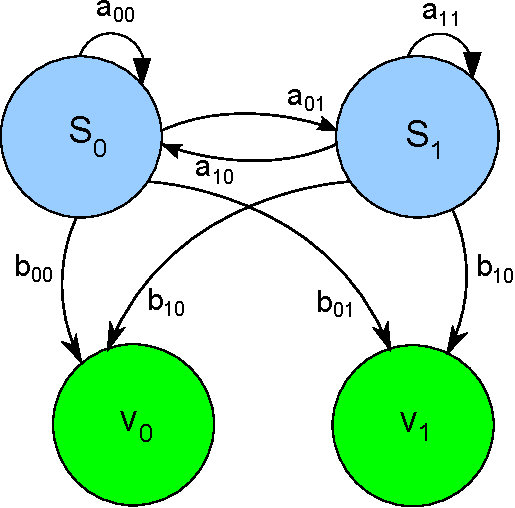
\includegraphics[width=0.5\textwidth]{figs/HMM_flowDiagram.pdf}
%	\caption{Visual tracking, overview}
%	\label{TRK_objectRepresentations}
%\end{figure}
%
%\begin{figure}[t]
%	\center
%	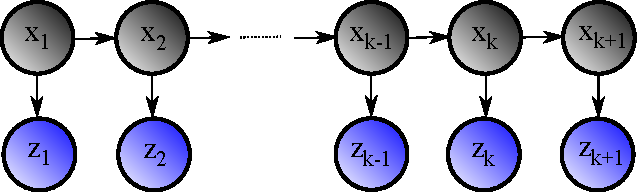
\includegraphics[width=0.5\textwidth]{figs/HMM_flowDiagram2.pdf}
%	\caption{Visual tracking, overview}
%	\label{TRK_objectRepresentations}
%\end{figure}

%########################
\section{Prior work}
\label{Sec:RVQ_prior_work}	
%########################
\begin{figure}[htp]	
\centering	
\subfigure[Training phase (left image), testing phase (right image).]{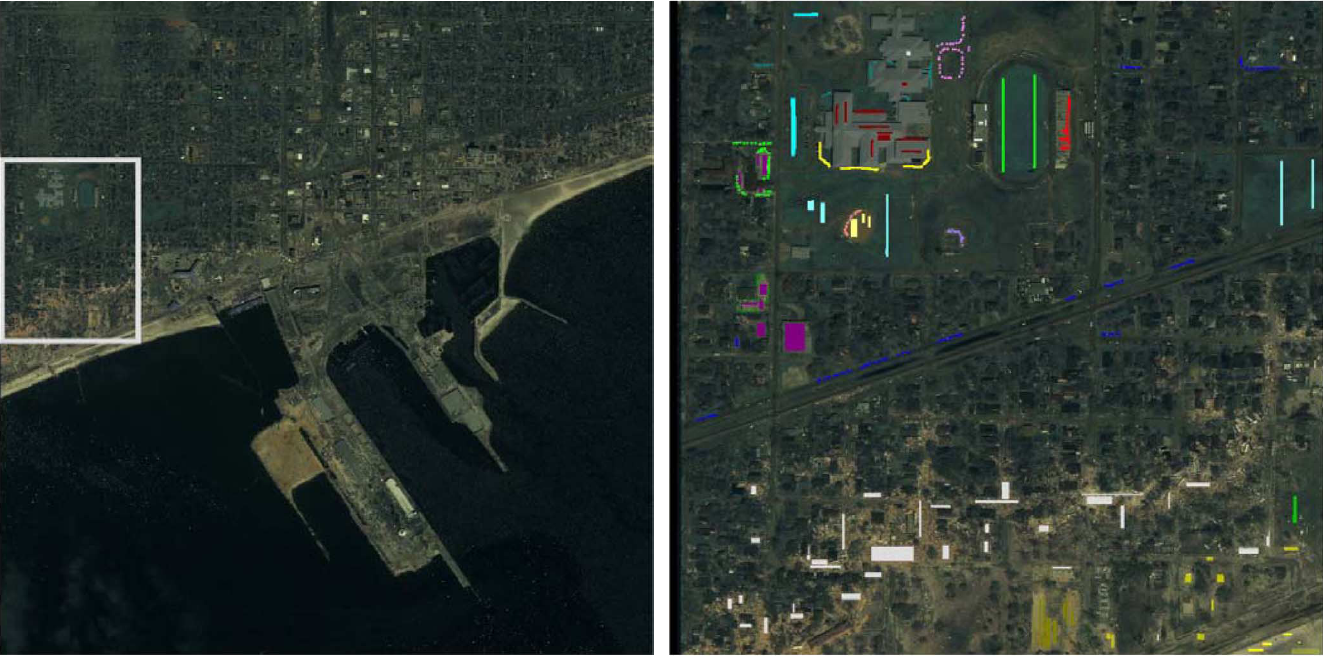
\includegraphics[width=0.7\textwidth]{figs/RVQ_SatelliteKatrina_1_snippets.png}}
\subfigure[RVQ $\sigma$ tree code-vectors.  Stages increase vertically, code-vectors per stage are laid out horizontally.]{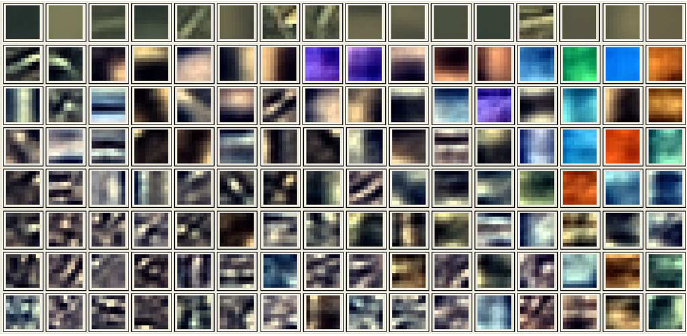
\includegraphics[width=0.5\textwidth]{figs/RVQ_SatelliteKatrina_2_codebooks.png}}
\caption{Disaster assessment, Hurricane Katrina, 2005.  In the top left image, window chips inside the white box are used as training image snippets for RVQ.  These image snippets are used to generate RVQ $\sigma$ tree code-vectors.  In the top right image, classification of various damaged structures is carried out \cite{2007_JNL_Katrina_Barnes}.}
\end{figure}

The first reported usage of RVQ for image analysis was reported in 2007 for damage assessment of the 2005 Hurricane Katrina~\cite{2007_JNL_Katrina_Barnes} and area assessment of the Payagala region in Sri Lanka before the 2007 Asian Tsunami~\cite{2007_JNL_IDDM_Barnes}.    

For Hurricane Katrina~\cite{2007_JNL_Katrina_Barnes}, high resolution satellite imagery in nearshore areas in the aftermath of Hurricane Katrina in Gulfport MS was investigated for damage assessments and emergency response planning.  It was shown that RVQ $\sigma$-trees have the capability to detect hurricane debris fields and storm-impacted nearshore features such as wind-damaged buildings, sand deposits, standing water, etc.  In addition, non-impacted features such as buildings, vegetation, roadways, railways, etc were also detected and classified.  Classification rates in excess of 80\% were reported in most cases which were for the most part, significantly higher than user generated classification rates. 

The method of employing RVQ in both~\cite{2007_JNL_Katrina_Barnes} and \cite{2007_JNL_IDDM_Barnes} is similar.  The number of examples $x_i$ from a particular class $\mathcal{C}_c$ that map to a particular RVQ stage code-vector $m_{t,c}$ in a $\sigma$-tree were added to create stage-wise counts,

\begin{equation}
N_{t,s,c} = \sum\limits_{i=1}^N\mathrm{I}(x_i \in \mathcal{C}_c, \mathbf{i}_{x_i}(t)=s)
\end{equation}

where $\mathrm{I}(.)$ is the indicator function, $\mathbf{i}_{x_i}$ is the XDR descriptor for $x_i$, $t$ is the stage index, $s$ is the stage code-vector index within the stage, $c$ is the class index, $N$ is the total number of training examples, and $\mathcal{C}_c$ is the $c$-th class.  These counts are sufficient statistics for the class conditional densities that are used for classification \cite{1993_BOOK_SSP_Kay}.

We extend this early work in RVQ image analysis to face recognition.  The goal is to understand RVQ in the context of image analysis a little better before it is applied to image sequence analysis.  The next section discusses the usage of RVQ for image sequence analysis in the context of action recognition.  With these two use cases covered, we will then approach the main topic of this research, that of using RVQ in image sequence analysis in the context of target tracking.

\begin{figure}
\centering
\includegraphics[width=0.6\textwidth]{figs/PRML_PCA_axis_rotation.pdf}
\caption{Axis rotation in $R^2$ in PCA.  $\mathrm{x}_1$ and $\mathrm{x}_2$ form the original basis.  The new rotated basis is formed by the vectors $\mathrm{z}_1$ and $\mathrm{z}_2$.  The data points are $x_i$, their projections on the new basis are $p_i$.  $e_i$ is the orthogonal projection error.}
\label{fig:PCA_axis_rotation}
\end{figure}

%
%\begin{equation}
%N = \sum\limits_{c=1}^C\sum\limits_{s=1}^{S} N_{t,s,c}, \ \ t = 1, 2, \ldots, T
%\end{equation}
%
%During the testing phase, the class label $c_{x_i}^*$ for a test point $x_i$ is computed as follows,
%\begin{equation}
%c_{x_i}^* \triangleq \mbox{arg}\max\limits_c   
%\bigg \{
%N_{1,\textbf{i}_{x_i}(1), c}, N_{2,\textbf{i}_{x_i}(2), c}, \ldots N_{T,\mathbf{i}_{x_i}(T), c}
%\bigg \} 
%\end{equation}
%
%In other words, the following steps are taken:
%
%\begin{itemize}
%\item Consider the path of $\mathbf{i}_{x_i}$ through the RVQ $\sigma$-tree, like the three example paths shown in Figure~\ref{fig:RVQ_2007_JNL_IDDM_Barnes_approach}
%\item Consider only the stage code-vectors in this path
%\item For each of these stage code-vectors, examine the counts for each class
%\item Pick the class with the highest count 
%\end{itemize}



%########################
\section{Face recognition}
%########################
Face recognition is an active area of research.  In this work, we carry out face recognition using RVQ and compare our results with two other well-known methods, PCA and SVM.  

%=====================
\subsection{PCA}
%=====================
The PCA based eigenface method for face recognition was first introduced in \cite{1991_JNL_Eigenfaces_Turk}.  In PCA the goal is to rotate the basis so as to maximize the variance of the projections.  This is shown graphically in Figure~\ref{fig:PCA_axis_rotation}.  A comparison of typical employment of PCA with another well-known method, Fourier analysis is shown in Figure~\ref{fig:PCA_Fourier_comparison}.



In PCA, the squared $L_2$ norm of the error $e_i$ between the data points $x_i$ and their projections $p_i$ can be computed as,

\begin{align}
x_i'x_i 		&= 	(e_i + p_i)'(e_i + p_i) \notag\\
		&=	e_i'e_i + p_i'p_i + 2e_i'p_i\notag\\
e_i'e_i		=&	x_i'x_i - p_i'p_i\notag\\
\sum\limits_{i=1}^{N}e_i'e_i		&=	\sum\limits_{i=1}^{N}x_i'x_i - \sum\limits_{i=1}^{N}p_i'p_i
\end{align}

\begin{figure}[tp]
\centering
\includegraphics[width=0.75\textwidth]{figs/PRML_PCA_blockDiagram.pdf}
\caption{Comparison of typical employment of Fourier and PCA analysis}
\label{fig:PCA_Fourier_comparison}
\end{figure}

Therefore, in order to minimize the projection error, we need to maximize the squared $L_2$ norm of the projections,

\begin{align}
\sum\limits_{i=1}^{N} p_i'p_i 				&= \sum\limits_{i=1}^{N} \mbox{tr}(p_ip_i')\notag\\
				&= \sum\limits_{i=1}^{N} \mbox{tr}(V_q'x_ix_i'V_q)\notag\\
				&= \mbox{tr} \left[ V_q' \left(\sum\limits_{i=1}^{N} (x_ix_i')\right) V_q \right]\notag\\
				&= \mbox{tr} (V_q'XX'V_q)\notag\\
				&= \mbox{tr} (V_q'\Sigma V_q)
\label{Eq:PCA_projections}
\end{align}

The quantity in Equation~\ref{Eq:PCA_projections} can be maximized by picking the matrix $V_q$ such that its columns are the eigenvectors of the covariance matrix $\Sigma$ of the input data points $x_i$~\cite{2002_BOOK_PCA_Jolliffe}.  In other words, the new basis that minimizes projection error is formed from the eigenvectors of the covariance matrix of the data.  This is the geometric derivation of PCA.  Refer to~\cite{2002_BOOK_PCA_Jolliffe} for a detailed explanation of both geometric and algebraic derivations.

%=====================
\subsection{SVM}
%=====================
								\begin{figure}[tp]
									\center
									\includegraphics[width=0.65\textwidth]{figs/PRML_discriminantFunction.pdf}
									\caption{Linear discriminant function}
									\label{PRML_discriminantFunction}
								\end{figure}

The second method that we compare RVQ to in the context of face recognition is Support Vector Machines (SVM).  

Figure~\ref{PRML_discriminantFunction} shows a linear discriminant function, $y(\mathbf{x})=0$, in $R^2$.  For two points, $\mathbf{x}_A$ and $\mathbf{x}_B$ that lie on this line,

\begin{equation}
\begin{array}{lll}
y(\textbf{x}_A)					&=		y(\textbf{x}_B)					&=0\\
\Rightarrow \mathbf{w}^T\mathbf{x}_A+b	&=		\mathbf{w}^T\mathbf{x}_B+b	&=0\\
\Rightarrow \mathbf{w}^T(\mathbf{x}_A-\mathbf{x}_B)			&=0\\
\Rightarrow \mathbf{w} \perp (\mathbf{x}_A-\mathbf{x}_B)\\
\end{array}
\label{Eqn:w_perp_LDF}
\end{equation}

Equation~\ref{Eqn:w_perp_LDF} means that the weight vector $\mathbf{w}$ is perpendicular to the linear discriminant function, $y(\mathbf{x})=0$.  

For a point $\mathbf{x}$ that does not lie on this line, simple vector addition gives,

\begin{equation}
\begin{array}{clllll}
\mathbf{x}		&=\mathbf{x}_{\perp} &&+ &r\frac{\mathbf{w}}{\|\mathbf{w}\|}\\
\Rightarrow \mathbf{w}^T\mathbf{x} +b		&=\mathbf{w}^T\mathbf{x}_{\perp} &+ b &+ &r \mathbf{w}^T \frac{\mathbf{w}}{\|\mathbf{w}\|}\\
y(\mathbf{x}) &= 0 && + &r\|\mathbf{w}\|\\
\Rightarrow r&=\frac{y(\mathbf{x})}{\|\mathbf{w}\|}
\end{array}
\label{Eqn:margin}
\end{equation}

In Equation~\ref{Eqn:margin}, $r$ is the \emph{margin}.  We are interested in the margin since we want to achieve the following two goals:

\begin{itemize}
\item \underline{Low \emph{risk}}.  This is equivalent to high correct training classification rate.  If the data is linearly separable, zero risk can be achieved whether the margin $r$ is low or high.
\item \underline{High \emph{generalization}}.  This is equivalent to high correct testing classification rate.  In order to achieve this goal, statistical learning theory tells us that the margin must be maximized~\cite{1996_BOOK_PR_DevroyeGyorfiLugosi}.
\end{itemize}

For the binary classification case with labels $t_n \in \{-1, 1\}$, the above goals are achieved if $t_ny(\mathbf{x}_n)>0, \ \forall n$.  The margin can therefore be rewritten as,

\begin{align}
r &= t_n\frac{y(\mathbf{x}_n)}{{\|\mathbf{w}\|}}\\\notag
&=t_n\frac{\mathbf{w}^T\mathbf{x}_n+b}{\|\mathbf{w}\|}
\end{align}

Using a general basis function $\phi(\mathbf{x}_n)$, the margin becomes

\begin{equation}
r = t_n\frac{\mathbf{w}^T\phi(\mathbf{x}_n)+b}{\|\mathbf{w}\|}
\end{equation}

We are interested in maximizing this margin to get good generalization, i.e., low test error.  The optimal solution for the discriminant function parameters $\mathbf{w}$ and $b$ is therefore,

\begin{equation}
\mathbf{w}^*, b^* = \arg \max_{\mathbf{w},b} \left[\frac{1}{{\|\mathbf{w}\|}}\ \ \min_n \ \ t_n\left(\mathbf{w}^T\phi(\mathbf{x}_n)+b\right)\right]
\end{equation}

Without loss of generality, we can set $t_n\left(\mathbf{w}^T\phi(\mathbf{x}_n)+b\right) = 1$ under the $N$ constraints that $t_n\left(\mathbf{w}^T\phi(\mathbf{x}_n)+b\right) \geq 1, \ n=1, 2, \ldots N$.  Therefore,  

\begin{equation}
\mathbf{w}^*, b^* = \arg \min_{\mathbf{w},b} {\|\mathbf{w}\|}
\end{equation}

											\begin{figure}[t]
											\centering
											\includegraphics[width=1.0\textwidth]{figs/RVQ_testingMethodsDensities.pdf}
											\caption{RVQ training phase, creating class conditional densities using first order Markov conditions on the training RVQ XDR descriptors.}
											\label{fig:RVQ_testingMethodsDensities}
											\end{figure}



Introducing Lagrange multipliers, $a_n \geq 0$ with one multiplier per constraint, gives the following Lagrangian function,

\begin{equation}
L(\mathbf{x}, b, \mathbf{a}) = \frac{1}{2}{\|\mathbf{w}\|}^2 - \sum\limits_{n=1}^N a_n \left[t_n\left(\mathbf{w}^T\phi(\mathbf{x}_n)+b\right)-1\right]
\label{Eqn:SVM_lagrange_function}
\end{equation}

where $\mathbf{a} = (a_1, a_2, \ldots, a_N)^T$.  Setting the derivative of $L(\mathbf{x}, b, \mathbf{a})$ with respect to $\mathbf{w}$ and $b$ equal to 0 gives the following two conditions

\begin{align}
\mathbf{w} &= \sum\limits_{n=1}^N a_n t_n \phi(\mathbf{x})\\
0 &=  \sum\limits_{n=1}^N a_n t_n
\end{align}

Eliminating $\mathbf{w}$ and $b$ from the Lagrange function $L(\mathbf{x}, b, \mathbf{a})$ in Equation~\ref{Eqn:SVM_lagrange_function} gives the \emph{dual} representation,

\begin{equation}
\tilde{L}(\mathbf{a}) = \sum\limits_{n=1}^N a_n - \frac{1}{2} \sum\limits_{n=1}^N \sum\limits_{m=1}^N a_n a_m t_n t_m k(\mathbf{x}_n, \mathbf{x}_m)
\label{Eqn:SVM_finalOptimization}
\end{equation}

with the constraints,

\begin{align}
a_n &\geq 0, \ \ \ \ \ \ \ \ \ \ \ \ n = 1, 2, \ldots, N \\
\sum\limits_{n=1}^N a_n t_n &= 0
\end{align}

In Equation~\ref{Eqn:SVM_finalOptimization}, $k(\mathbf{x}, \mathbf{x}') = \phi(\mathbf{x})^T\phi(\mathbf{x}')$ is a kernel function \cite{2007_BOOK_PRML_Bishop}.  The solution to this quadratic programming problem gives the maximum margin discriminant function.  Using kernels in the SVM formulation allows for linear discriminant functions in higher dimensional spaces and corresponding non-linear discriminant functions in the original data space.  An example of this is given in Figure~\ref{fig:SVM_kernel_example} \cite{2007_VID_kernel_Scholkpof}.

								\begin{figure}[t]
								\centering
								\subfigure[Data that is not linearly separable in $R^2$.]{\includegraphics[width=0.45\textwidth]{figs/kernel_input.pdf}}
								\subfigure[Projecting data from $R^2$ to $R^3$ using $(x',y',z') = (x^2, \sqrt(2)xy, y^2)$]{\includegraphics[width=0.45\textwidth]{figs/kernel_output.pdf}}
								\caption{Projecting from $R^2$ to $R^3$ causes data to become linearly separable in $R^3$.  The separating linear hyperplane in $R^3$ is projected down to a non-linear ellipse in $R^2$.}
								\label{fig:SVM_kernel_example}
								\end{figure}






%===========================
\subsection{RVQ}
\label{subsec:RVQ}
%===========================
The general methodology for face recognition using the two algorithms previously discussed is,

\begin{itemize}
\item \underline{PCA}: Two commonly used metrics are reconstruction error and Euclidean distance between face projections on the first few principal components.
\item \underline{SVM}: Multi-class SVM treats face recognition as a multi-class classification problem.  
\end{itemize}
								\begin{figure}[t]
								\centering
								\includegraphics[width=1.0\textwidth]{figs/RVQ_2007_JNL_IDDM_Barnes_approach.pdf}
								\caption{RVQ training phase, mapping input data points to various stage code-vectors in the RVQ $\sigma$-tree.  The yellow circles represent stage code-vectors.  The black arrows represent possible paths for the data through the RVQ $\sigma$ tree.  The most likely paths for data points belonging to classes $\mathcal{C}_1$, $\mathcal{C}_2$ and $\mathcal{C}_C$ are also shown.}
								\label{fig:RVQ_2007_JNL_IDDM_Barnes_approach}
								\end{figure}



In RVQ, a number of methods can be used to find the class to which an test data point $x_i$ should be assigned to based on its XDR:

\begin{enumerate}
\item \underline{Squared error on XDR converted to a scalar value}.  The RVQ descriptor $\mathbf{i}$, called XDR (expanded digital representation) \cite{2007_JNL_IDDM_Barnes} is a $T$-tuple for a $T$x$S$ RVQ $\sigma$-tree in which the $t$-th entry corresponds to the index of a mapped stage code-vector at the $t$-th stage.  
							\begin{figure}[t]
							\centering
							\includegraphics[width=1.0\textwidth]{figs/RVQ_bayesNet.pdf}
							\caption{RVQ testing phase, testing an XDR $\mathbf{i}$ against the $c$-th class $\mathcal{C}_c$}
							\label{fig:RVQ_bayesNet.pdf}
							\end{figure}




	\begin{itemize}
		\item The XDR $\mathbf{i}$ can be converted to a scalar values $\iota$ using the following invertible mapping,
\begin{equation}
\iota=\sum\limits_{t=1}^{T}\mathbf{i}(t)S^{(T-t)}
\end{equation}
		\item This is a geometric weighting of the components of the XDR $T$-tuple.  The first stage is weighted the most, followed by geometrically decreasing weights for the subsequent stages.  If there is only one code-vector per stage, $\iota$ is the sum of every stage code-vector.  For an 8x2 RVQ $\sigma$-tree, i.e. 8 stages and 2 code-vectors per stage, $\iota$ ranges from 0 to 255, and a single byte is required to represent it.
		\item The distance between 2 XDR's, $\mathbf{i}_A$ and $\mathbf{i}_B$ is then simply, 
\begin{equation}
d = \bigg|\sum\limits_{t=1}^{T}\mathbf{i}_A(t)S^{(T-t)} - \sum\limits_{t=1}^{T}\mathbf{i}_B(t)S^{(T-t)}\bigg|
\end{equation}
	\item A test XDR $\mathbf{i}$ can be compared to XDRs of all training data points using this method.  A class is then assigned to $\mathbf{i}$ which is the same as the class of the training data point whose XDR distance is the least.
	\end{itemize}

								\begin{figure}[t]
								\includegraphics[width=1.0\textwidth]{figs/PRML_PCA_faceRecognition_1_trainingFaces.png}
								\caption{Training images, Yale face dataset}
								\label{fig:dataset_Yale}
								\end{figure}

\item \underline{Hamming distance on XDR}.  The distance between two XDRs can be represented as a Hamming distance,
\begin{equation}
d_H = \sum\limits_{t=1}^{T}\mathrm{I}\bigg(\mathbf{i}_A(t) \neq \mathbf{i}_B(t)\bigg)
\end{equation}
where $\mathrm{I}(.)$ is the indicator function.  Again, a class is then assigned to $\mathbf{i}$ which is the same as the class of the training data point whose XDR distance is the least.
\item \underline{Class-conditional probabilities}.  
\begin{enumerate}


											\begin{figure}[t]
											\centering
											\subfigure[]{\includegraphics[width=0.1\textwidth]{figs/PRML_PCA_faceRecognition_3_averageFace.png}}
											\subfigure[]{\includegraphics[width=0.9\textwidth]{figs/PRML_PCA_faceRecognition_6_eigenFaces.png}}
											\caption{PCA (a) average face, (b) eigenfaces, for the Yale face dataset.}
											\label{fig:PCA_eigenfaces_Yale}
											\end{figure}

\item \underline{Training phase}.  If training data is available, then class conditional densities can be generated using the transitions of the XDR $T$-tuple.  On the one extreme, it can be assumed that each entry in the XDR $T$-tuple depends on every other entry.  Although correct, given the CAC condition discussed in Chapter~\ref{chap_RVQ}, this would make the joint density intractable.  The other extreme is assuming complete independence between all entries of the XDR $T$-tuple.  This would cause the joint density to factor into marginal densities but this assumption is too relaxed.  In the middle ground, different order Markov conditions can be assumed that would allow the joint density to factor into conditional densities.  For simplicity and to avoid combinatorial complexity, we choose to pick a first order Markov condition as shown in Figure~\ref{fig:RVQ_testingMethodsDensities}.  In this figure, $X_t$ is the random variable for the $t$-th stage that takes on values $1, 2, \ldots, S$, i.e. indeces of stage code-vectors for the training XDRs.  For $T$ stages and $C$ classes, a total of $C(T-1)$ class conditional densities are generated.  As mentioned in Section~\ref{Sec:RVQ_prior_work}, the sufficient statistics for these class-conditional densities are stage counts \cite{1993_BOOK_SSP_Kay}.  In a manner similar to the prior work on RVQ~\cite{2007_JNL_Katrina_Barnes, 2007_JNL_IDDM_Barnes}, a stage count $N_{t,s,c}$ is the number of training examples in the $c$-th class that map to stage code-vector $s$ at stage $t$.  This is depicted graphically in Figure~\ref{fig:RVQ_2007_JNL_IDDM_Barnes_approach}.  The number of training examples that are input at every stage $t$,  is the same, i.e. $N$,

											\begin{figure}[t]
											\center
											\includegraphics[width=0.7\textwidth]{figs/PCA_comparison.pdf}
											\caption{PCA face recognition results.}
											\label{fig:PCA_yaleface_results}
											\end{figure}


\begin{equation}
N = \sum\limits_{c=1}^C\sum\limits_{s=1}^{S} N_{t,s,c}
\end{equation}

This is in contrast to TSVQ where in general, the number of examples that are used to create a  code-vector at a particular stage reduces from the prior stage.  The class conditional densities are generated using these counts
To go from class counts to class conditional densities, Lidstone Law is used to assign a small probability to paths through the RVQ $\sigma$-tree that are not visited during training as follows,

									\begin{figure}[t]
									\centering
									\subfigure{\includegraphics[width=0.23\textwidth]{figs/SVM_yaleFace_linearKernel_3Dsurf.pdf}}
									\subfigure{\includegraphics[width=0.23\textwidth]{figs/SVM_yaleFace_polynomialKernel_3Dsurf.pdf}}
									\subfigure{\includegraphics[width=0.23\textwidth]{figs/SVM_yaleFace_RBFkernel_3Dsurf.pdf}}
									\subfigure{\includegraphics[width=0.23\textwidth]{figs/SVM_yaleFace_sigmoidKernel_3Dsurf.pdf}}
									\subfigure{\includegraphics[width=0.23\textwidth]{figs/SVM_yaleFace_linearKernel_2D.pdf}}
									\subfigure{\includegraphics[width=0.23\textwidth]{figs/SVM_yaleFace_polynomialKernel_2D.pdf}}
									\subfigure{\includegraphics[width=0.23\textwidth]{figs/SVM_yaleFace_RBFkernel_2D.pdf}}	
									\subfigure{\includegraphics[width=0.23\textwidth]{figs/SVM_yaleFace_sigmoidKernel_2D.pdf}}	
									\subfigure[Linear: 90\%]{\includegraphics[width=0.23\textwidth]{figs/SVM_yaleFace_linearKernel_hist.pdf}}
									\subfigure[Polynomial: 83\%]{\includegraphics[width=0.23\textwidth]{figs/SVM_yaleFace_polynomialKernel_hist.pdf}}
									\subfigure[RBF: 90\%]{\includegraphics[width=0.23\textwidth]{figs/SVM_yaleFace_RBFkernel_hist.pdf}}
									\subfigure[Sigmoid: 93\%]{\includegraphics[width=0.23\textwidth]{figs/SVM_yaleFace_sigmoidKernel_hist.pdf}}
									\caption{SVM face recognition rates for the Yale dataset for different values of the cost parameter $C_{svm}$ and kernel parameter $\gamma$.  Top row, L to R, kernels: linear (90\%), polynomial (83\%), RBF (90\%), sigmoid (93\%).  The middle row is the 2D equivalent plot for the top row shown for better visualization.  Bottom row, face recognition accuracies for the 399 possible combinations of $C_{svm}$ and $\gamma$ values.  Notice that the linear kernel does not depend on $C_{svm}$ and $\gamma$ but is shown to make the plots look uniform for better comparison.}
									\label{fig:SVM_yaleface_results}
									\end{figure}



\begin{equation}
p(X_t=x_t) = \frac{\sum\limits_{n=1}^{N}I(X_t=x_t)+\lambda}{N+\lambda S}, \ \ x_t \in \{1, 2, \dots, S\}
\end{equation}
  
In the equation above, $\lambda=0$ corresponds to the maximum likelihood estimate (MLE), $\lambda=0.5$ corresponds to the Jeffrey-Perks Law and $\lambda=1$ corresponds to Laplace's Law.
\item \underline{Testing phase}.  During the testing phase, the probability of an input data point $\mathbf{x}_i$ with corresponding XDR $\mathbf{i}_i$ belonging to class $\mathcal{C}_c$ is given by,

\begin{equation}
\begin{array}{llllll}
p (\mathbf{i}_i|\mathcal{C}_c) &=& p \bigg (\mathbf{i}_n(T) \ | \ \mathbf{i}_i(T-1), \mathcal{C}_c \bigg) \ . \ 
p \bigg(\mathbf{i}_i(T-1) \ | \ \mathbf{i}_i(T-2), \mathcal{C}_c \bigg) \ldots  
p \bigg (\mathbf{i}_i(1) \ | \ \mathcal{C}_c \bigg ) \\
\end{array}
\end{equation}
									\begin{figure}[t]
									\centering
									\subfigure[8x2]{\includegraphics[width=0.20\textwidth]{f:/salman/PhDold/figs/new/RVQ_yaleFaces_dcbk_M_2-8.jpg}}
									\subfigure[8x3]{\includegraphics[width=0.30\textwidth]{f:/salman/PhDold/figs/new/RVQ_yaleFaces_dcbk_M_3-8.jpg}}
									\subfigure[8x4]{\includegraphics[width=0.40\textwidth]{f:/salman/PhDold/figs/new/RVQ_yaleFaces_dcbk_M_4-8.jpg}}
									\caption{RVQ codebooks for the Yale face dataset, number of code-vectors per stage is much less than the number of classes, $S << C$}
									\label{fig:RVQ_codebooks_smallS_Yale}	
									\end{figure}



This is shown graphically in Figure~\ref{fig:RVQ_bayesNet.pdf}.  The class with the highest probability is picked.
\end{enumerate}
\end{enumerate}

%===========================
\subsection{Results}
%===========================
									\begin{figure}[t]
									\centering
									\includegraphics[width=1.0\textwidth]{f:/salman/PhDold/figs/new/RVQ_yaleFaces_dcbk_M_15-8.png}
									\caption{RVQ codebooks for the Yale face dataset, number of code-vectors per stage is equal to the number of classes, $S=C$}
									\label{fig:RVQ_codebooks_largeS_Yale}	
									\end{figure}

In this work, we use a commonly used dataset for face recognition, the Yale dataset as shown in Figure~\ref{fig:dataset_Yale}.  This dataset has 11 images each of 15 individuals.  For PCA, SVM and RVQ, we use the leave-one-out cross validation method since the number of training images is limited.  

For PCA, the test image $\mathbf{x}_t$ is projected on the PCA basis $\mathbf{U}$ to get its eigenvalue projections.  The Euclidean distance between a subset of these projections and the projections of the remaining training images belonging to all classes, $x_{c,i}, \  i=1, 2, \ldots N, \ c=1, 2, \ldots, C$ is compared.  The class $c^*_{x_t}$ of that training image is picked which gives the least Euclidean error,


\begin{equation}
c^*_{x_t} = \arg\min_c\|U^Tx_t - U^Tx_{c,i}\| \ \ \  i=1, 2, \ldots N, \ \ c=1, 2, \ldots, C
\end{equation}

Figure~\ref{fig:PCA_eigenfaces_Yale} shows the results of this operation with different numbers $q$ of eigenvectors retained from the PCA basis $\mathbf{U}$.  Retained eigenvectors start from the principal component, i.e. the basis vector that had the highest variance for the projections of the training data, and proceed in order with monotonically decreasing variances until $q$ eigenvectors have been retained.  No attempt is made to use any other order, or to retain $q$ eigenvectors by not starting the retention process at the first principal component.  The reason is that the goal is to attempt an apples-to-apples comparison with SVM and RVQ and it is not clear how the effects of such operations in PCA could be duplicated in the other algorithms.  The leave-one-out cross-validation procedure leads to 165 iterations of the algorithm.  Figure~\ref{fig:PCA_eigenfaces_Yale} shows that the highest classification accuracy averaged over these 165 iterations is 80\%.  Only 40 out of the possible 165 eigenvectors are needed to to achieve this.  However, even 15 eigenvectors, i.e. 11\% of the maximum possible, can be retained to get around 78\% correct recognition rate.  PCA eigenfaces are shown in Figure~\ref{fig:RVQ_eigenfaces_Yale}.

											\begin{figure}[t]
											\centering
											\subfigure[S=2]{\includegraphics[width=0.2\textwidth]{figs/RVQ_yaleFaces_decimal_ptuples_M-2.png}}
											\subfigure[S=3]{\includegraphics[width=0.2\textwidth]{figs/RVQ_yaleFaces_decimal_ptuples_M-3.png}}
											\subfigure[S=4]{\includegraphics[width=0.2\textwidth]{figs/RVQ_yaleFaces_decimal_ptuples_M-4.png}}
											\subfigure[S=5]{\includegraphics[width=0.2\textwidth]{figs/RVQ_yaleFaces_decimal_ptuples_M-5.png}}
											\subfigure[S=6]{\includegraphics[width=0.2\textwidth]{figs/RVQ_yaleFaces_decimal_ptuples_M-6.png}}
											\subfigure[S=7]{\includegraphics[width=0.2\textwidth]{figs/RVQ_yaleFaces_decimal_ptuples_M-7.png}}
											\subfigure[S=8]{\includegraphics[width=0.2\textwidth]{figs/RVQ_yaleFaces_decimal_ptuples_M-8.png}}
											\caption{RVQ training, scalar XDR for the training images.  The scalar XDR $\iota$ is created through an invertible mapping from the $T$-tuple XDR $\mathbf{i}$, $\iota=\sum\limits_{t=1}^{T}\mathbf{i}(t)S^{(T-t)}$.  In these images, the number of stages $T=8$.  The x-axis goes from 0 to 163 for the 164 training images.  One image has been left out due to cross-one-out cross-validation.  The y-axis is the value of the scalar XDR.}
											\label{fig:RVQ_faceRecognition_sSoC}	
											\end{figure}

For SVM, the software library \emph{libSVM} was used \cite{2011_JNL_libSVM_Chang}.  The following four SVM kernels were tested, 

\begin{equation}
\begin{array}{lllllll}
\mathrm{linear:} & k(\mathbf{x}_i, \mathbf{x}_j) &= \mathbf{x}_i \cdot \mathbf{x}_j\\ 
\mathrm{polynomial:} & k(\mathbf{x}_i, \mathbf{x}_j) &= (\gamma \ \mathbf{x}_i \cdot \mathbf{x}_j)^3\\
\mathrm{RBF:} & k(\mathbf{x}, \mathbf{x'}) &= \exp(-\gamma \ \|\mathbf{x}_i - \mathbf{x}_j\|^2)\\
\mathrm{Sigmoid:} & k(\mathbf{x}, \mathbf{x'}) &= \tanh(\gamma \ \mathbf{x}_i \cdot \mathbf{x}_j)\\
\end{array}
\end{equation}


											\begin{figure}[t]
											\centering
											\subtable[tabular results]{\input{f:/salman/PhDold/tables/RVQ_yaleFaces_dcbk_dSNR_achieved} }
											\subfigure[results above shown 2D graphically]{\includegraphics[width=0.45\textwidth]{figs/RVQ_faceRecognition_dSNR_2D.pdf}\label{fig:RVQ_faceRecognition_dSNR_2D}}
											\subfigure[results above shown 3D graphically]{\includegraphics[width=0.45\textwidth]{figs/RVQ_faceRecognition_dSNR_3D.pdf}\label{fig:RVQ_faceRecognition_dSNR_3D}}
											\caption{RVQ training on the Yale face dataset, training set reconstruction SNR (dB).}
											\label{fig:RVQ_trg_reconstruction_SNR}	
											\end{figure}

A grid search was done over values of the cost parameter $C_{svm}$ and kernel parameter $\gamma$ as is accepted practice.  $C_{svm}$ was allowed to take on values in $\{2^{-5}, 2^{-4} \ldots 2^{15}\}$, i.e. 21 distinct points.  The kernel parameter $\gamma$ was allowed to take on values in $\{2^{-15}, 2^{-14} \ldots 2^{3}\}$, i.e., 19 distinct points.  The total number of points searched was therefore 21 x 19 = 399.  Combined with 165 iterations due to the leave-one-out cross-validation method meant 165x399 $\approx$ 65,000 iterations per kernel.  Results of these experiments for face recognition using the Yale dataset are given in Figure~\ref{fig:SVM_yaleface_results}.  Notice that the highest face recognition accuracy achieved is with the sigmoid kernel.  At 93\%, it is significantly higher than the recognition accuracy achieved with PCA.  However, the grid search that resulted in finding this optimal SVM configuration, i.e. combination of $C_{svm}$ and $\gamma$, came at a significantly higher computational cost.  Also, few configurations of the sigmoid kernel result in high accuracy rates.  The lowest recognition accuracy is produced by the polynomial kernel, and it is also quite sensitive to configuration.  The RBF kernel is able to produce high recognition accuracies up to 90\% for several combinations of $C_{svm}$ and $\gamma$.  However, the linear kernel seems to be the best kernel to use in this case since it is able to produce 90\% recognition accuracy with little computational cost.

											\begin{figure}[t]
											\centering
											\subtable[tabular results]{\input{f:/salman/PhDold/tables/RVQ_yaleFaces_final}}
											\subfigure[graphical results]{\includegraphics[width=0.5\textwidth]{figs/RVQ_yaleFace_classifications2.pdf}}
											\caption{RVQ face recognition results}
											\label{fig:RVQ_yaleface_results}
											\end{figure}


For RVQ, Figure~\ref{fig:RVQ_faceRecognition_sSoC} shows values of scalar XDR for the training images for different values of numbers of code-vectors per stage, $S$.  The number of stages $T$ is fixed at 8.  Training images from a single class are placed next to each other and given the same color.  For zero risk, the amplitudes of a single class should all lie in a contiguous range with no overlap with the range of any other class.  The image shows that while several training examples satisfy this requirement, there are a few ambiguities.  It is therefore expected that we will have some generalization error.

RVQ codebooks for small values of code-vectors per stage are shown in Figure~\ref{fig:RVQ_codebooks_smallS_Yale}.  Here, the top-level code-vectors are somewhat blurred since most of them are combinations of one or more images from different classes.   In Figure~\ref{fig:RVQ_codebooks_largeS_Yale} where the number of stage code-vectors $S$ is equal to the number of classes $C$, the top-level stage code-vectors are in general, and as expected, less blurry and represent distinct classes.

Figure~\ref{fig:RVQ_trg_reconstruction_SNR} shows reconstruction SNR in dB for training set images based on the codebooks, some examples of which are given in Figures~\ref{fig:RVQ_codebooks_smallS_Yale} and~\ref{fig:RVQ_codebooks_smallS_Yale}.  As expected, the SNR increases as the number of stages $T$ or the number of code-vectors per stage $S$ increase.

Face recognition results for RVQ using all 3 methods mentioned in Section~\ref{subsec:RVQ} are given in Figure~\ref{fig:RVQ_yaleface_results}.  In general, the maximum likelihood method with Laplace Smoothing works best.  It also entails more computations.  12 configurations of RVQ are tested, 8x2, 8x3, 8x4, $\ldots$ 8x13.  Recognition results are averaged over all 165 images using cross-one-out cross-validation.  The results show that recognition rates improve as the number of code-vectors per stage is increased.  However that levels off after 8x4.  One would expect results to continue to improve.  However, the following two reasons are suspected to account for this behavior:

\begin{enumerate}
\item \underline{Design difficulty.}  As the number of code-vectors per stage increases, the complexity of the coupled K-means algorithms also increases.
\item \underline{Mean squared error not suitable criterion for face recognition.}  All VQ methods attempt to minimize mean squared reconstruction error.  It is not clear if minimizing mean squared error is the best methodology for face recognition and classification in general.  In contrast, SVM attempts to maximize classification margin, a method well suited to increasing classification accuracy.
\end{enumerate}

In comparing with PCA, RVQ using 8 stages and PCA using 8 eigenvectors have nearly the same recognition accuracy (72\% vs 73\% respectively).  Although it is not clear how to directly compare RVQ with PCA, comparing ESVQ (K-means) with PCA is more straightforward.  It is shown in \cite{2004_CNF_KmeansVsPCA_DingHe} that the K clusters produced by K-means (ESVQ) lie in the K-1 dimensional subspace generated by PCA.  One would therefore expect the following,

									\begin{figure}[t]
									\centering	
									\subfigure[Original images]{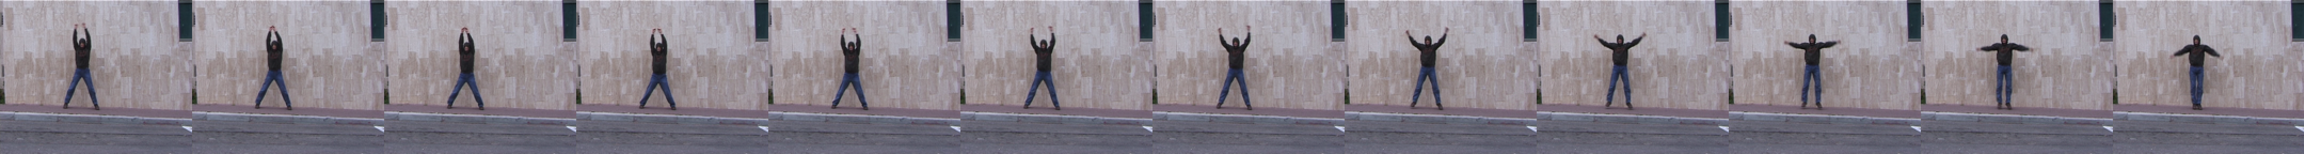
\includegraphics[width=1.0\textwidth]{figs/Proposal_fig5_RVQ_HMM_Weizmann_dataset_whole.png}}
									\subfigure[Segmented foreground]{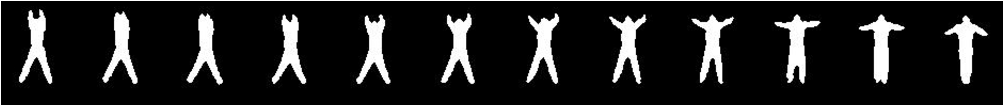
\includegraphics[width=1.0\textwidth]{figs/Proposal_fig5_RVQ_HMM_Weizmann_dataset.png}}\\
									\caption{Sample images from the Weizmann dataset for human action recognition~\cite{2007_JNL_SpaceTimeShapes_Gorelick}.}							
									\label{fig:Weizmann_sequence}				
									\end{figure}



\begin{enumerate}
\item \underline{Classification rates on linear manifolds.}  Since PCA is the optimal linear algorithm for mean squared error reconstruction, one would expect classification rates on linear manifolds for PCA and an optimal ESVQ to be the same.  
\item \underline{Classification rates on non-linear manifolds.}  On non-linear manifolds, an optimal ESVQ can produce less reconstruction error than PCA.  However, classification accuracy will depend on whether mean squared error is a good criterion for the dataset being used.
\end{enumerate}

Coming back to RVQ, for a given number of equivalent code-vectors, RVQ can at best match the reconstruction error of ESVQ.  However, since RVQ allows for an exponential number of equivalent code-vectors, it is possible for RVQ to get better reconstruction error than ESVQ with a $\sigma$-tree in which the number of stage code-vectors equals the number of code-vectors in ESVQ.  Based on this, for a dataset in which the mean squared error criterion leads to better classification, one would expect the classification/recognition accuracy of a properly designed RVQ to be equal than or more than that of PCA.  For this particular dataset, it is almost equal.  

We now turn to other scenarios to explore the behavior of RVQ.  In the next section, we look at action recognition in image sequences.  In the next chapter, we look at tracking in image sequences.


%\begin{equation}
%\mathcal{T}_{\mathrm{trg}}=  \{x_n \ \in R^D, n=\{1,2,\ldots, N\}\}
%\end{equation}
%
%to train the RVQ codebook.  The steps for this have been detailed in the preceding sections.  Once the codebook is trained, the resulting code-vectors can be used to represent data points that are not part of the training set.  Consider a test of $F$ test data points, 
%
%\begin{equation}
%\mathcal{T}_{\mathrm{tst}}=  \{x_f \ \in R^D, f=\{1,2,\ldots, F\}\}
%\end{equation}
%
%The goal is to represent $x_f$ in one of two possible ways:
%
%\begin{itemize}
%\item Existing code-vectors $\mu_k$.  In this method, a test input $x_f$ is tested against 
%
%\begin{equation}
%\textbf{i}_1 = \mathrm{arg} \min_i
%\end{equation}
%\item
%\end{itemize}


%\begin{align}
%p(\mathbf{X}|\mathcal{C}_c)  &=  p{(X_1, X_2, \ldots, X_T|\mathcal{C}_c)}\\\notag
%&= p(X_1|\mathcal{C}_c)p(X_2|X_1, \mathcal{C}_c)p(X_3|X_2, \mathcal{C}_c) \ldots p(X_T|X_{T-1}, \mathcal{C}_c) \\\notag
%&= \Pi_{t=1}^T p(X_t|X_{t-1}, \mathcal{C}_c) \\\notag
%\log p(\mathbf{X}|\mathcal{C}_c)&=\sum\limits_{t=1}^T \log p(X_t|X_{t-1}, \mathcal{C}_c)
%\end{align}

								\begin{figure}[t]		
								\includegraphics[width=1.0\textwidth]{figs/HMM}
								\caption{Discrete Hidden Markov Model (HMM), $N$ states, $M$ discrete observation symbols per state}
								\label{fig:HMM}
								\end{figure}


%########################
\section{Action recognition}
%########################
Usage of RVQ for human action recognition is first reported in Aslam et. al. \cite{2010_CNF_HMMRVQ_Aslam}.  We next explain the approach used.

Action recognition in images involves identifying the physical actions of humans from image sequences.  Typically, a subset of the possible set of human actions is used.  Widely used human actions include walking, running, jumping, skipping, waving and bending. 

The area of human action recognition has recently received a lot of attention.  A number of surveys are available on this topic \cite{1995_JNL_SURVEYmotion_Cedras, 1999_JNL_SURVEYmotion_Aggarwal, 1999_JNL_SURVEYmotion_Gavrila, 1999_REP_SURVEYmotion_Moeslund, 2001_JNL_SURVEYmotion_Moeslund, 2003_JNL_SURVEYiu_Buxton, 2003_JNL_SURVEYmotion_LWang, 2003_JNL_SURVEYbeh_Shah,2003_JNL_SURVEYaction_JWang, 2004_CNF_SURVEYaction_Aggarwal, 2004_JNL_SURVEYiu_Hu, 2004_CNF_SURVEYgait_Nixon, 2004_CNF_Survey3DshapeRetrieval, 2006_JNL_HumanMotion_Moeslund, 2007_JNL_HumanMotion_Poppe, 2008_CNF_SurveyHumanActivityRecognition_Ahad, 2010_JNL_SURVEYmotion_Ji}.  Bobick et al. \cite{2001_JNL_MotionTemplates_Bobick} introduced the notion of 2D templates of human action.  This was extended to 3D by Gorelick et al. \cite{2007_JNL_SpaceTimeShapes_Gorelick}.  Recently an approach based on kinematic features of 3D motion was used to recognize human action \cite{2010_JNL_ActionReconKinematic_Ali}.   

								\begin{figure}[t]
								\centering
								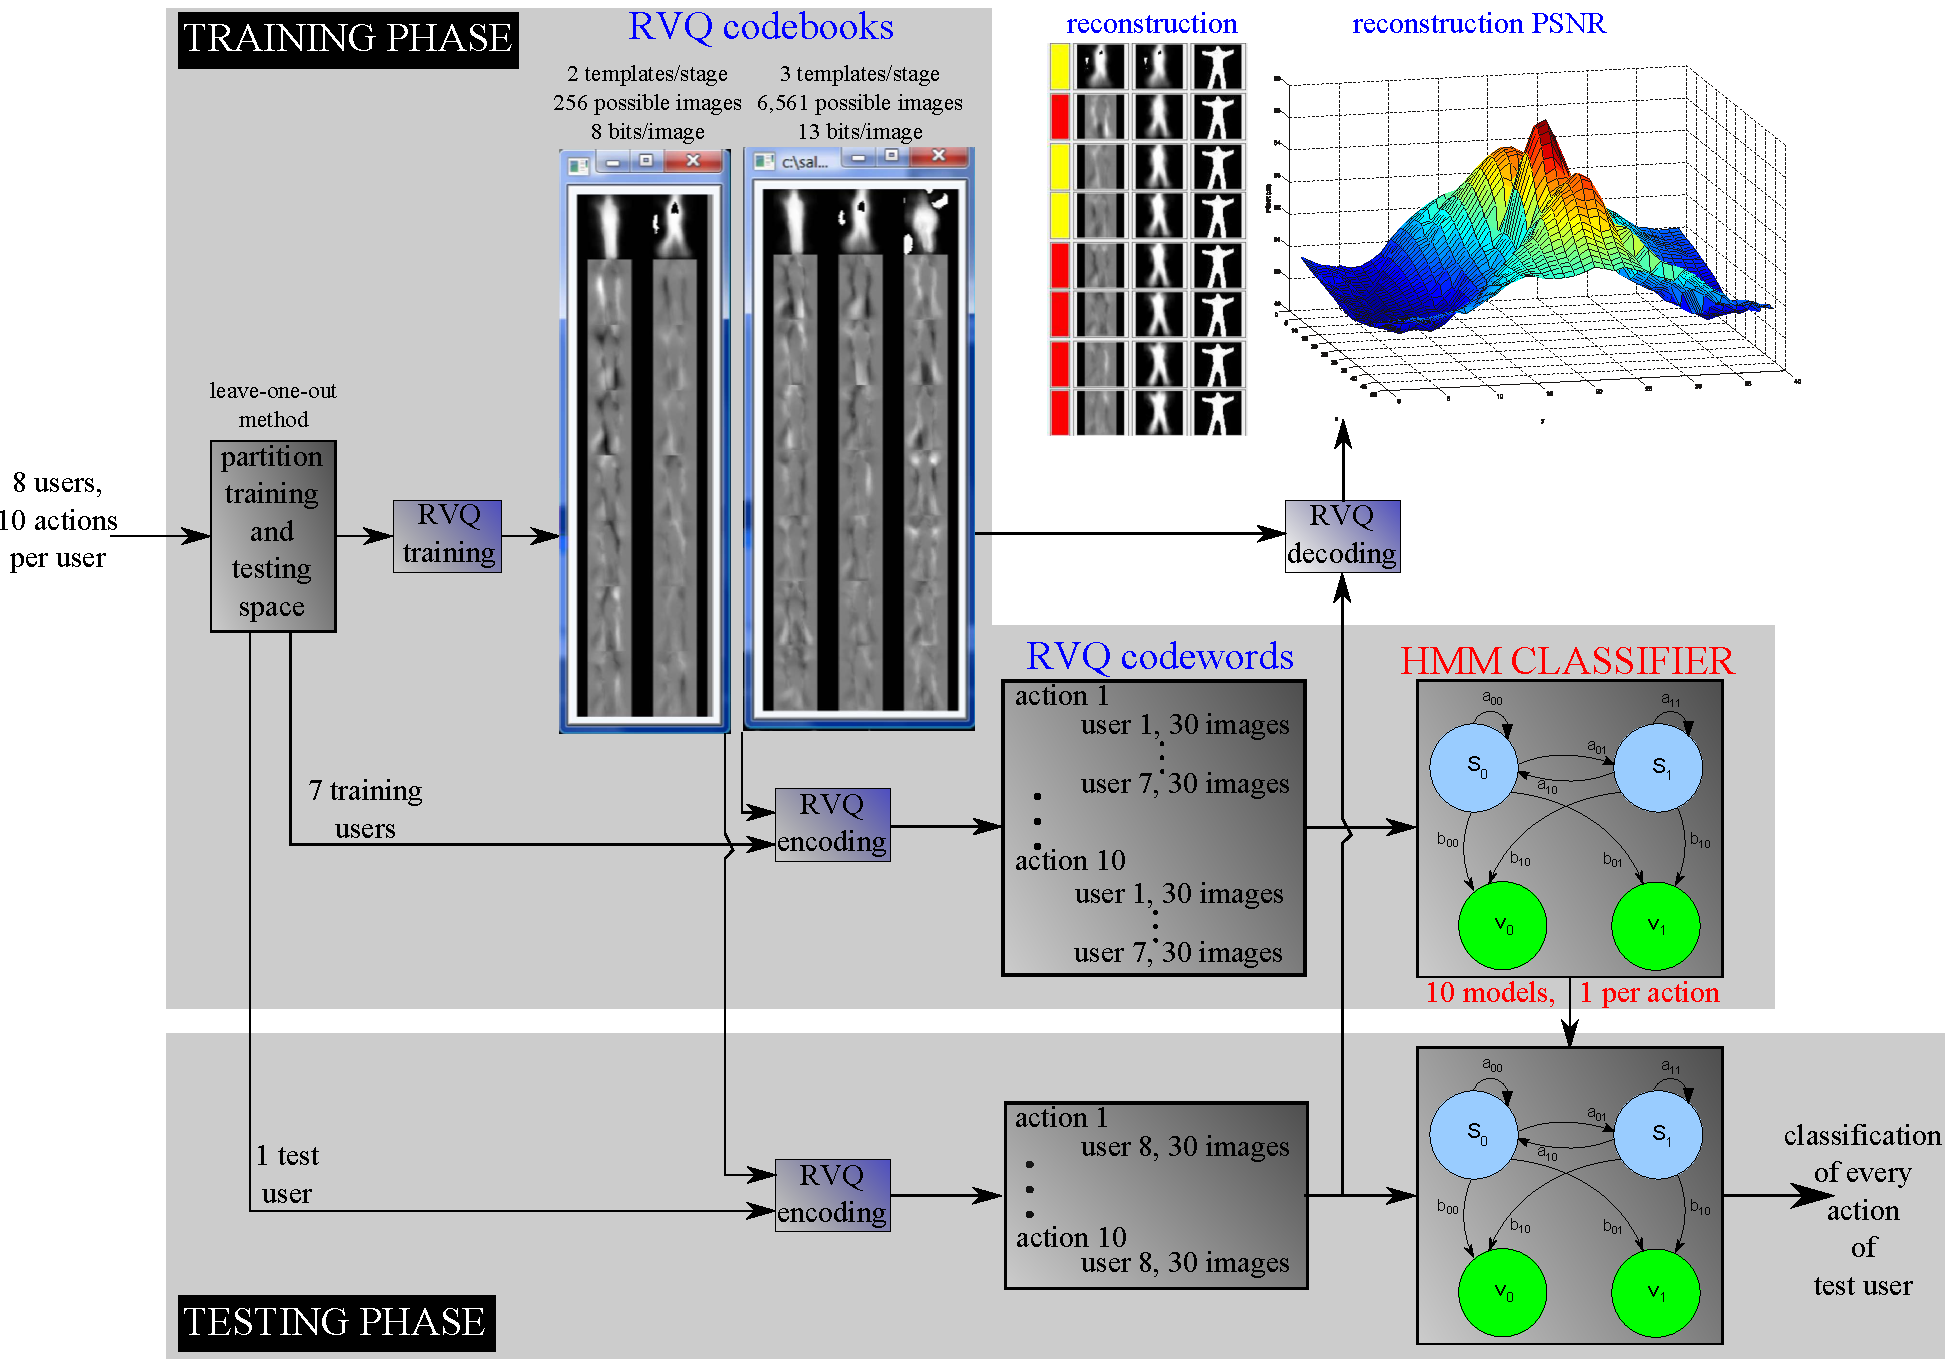
\includegraphics[width=1.0\textwidth]{figs/RVQ_HMM_IPCV2010_blockDiagram.pdf}
								\caption{Action recognition using RVQ, overall approach.}
								\label{fig:RVQ_HMM_IPCV2010_blockDiagram}
								\end{figure}


Our approach to tackling this problem is similar to \cite{2007_JNL_SpaceTimeShapes_Gorelick} in the sense that extracted features are used for classification using a simple Euclidean distance measure.  

In this work, we use the Weizmann dataset, a commonly used dataset for human action recognition.  We have a total of 8 users with the following 10 actions per user: (a) bending, (b) jumping jacks, (c) jumping, (d) in-place jumping (called \emph{pjump}), (e) running, (f) sideways jumping (called \emph{side}), (g) skipping, (h) walking, (i) one hand waving (called \emph{wave1}), and (j) two hand waving (called \emph{wave2}).  Each action is captured at 50 Hz and there are about 100 images per action, or 2 sec of video per action.  Our approach involves the use of Hidden Markov Models (HMMs).  We first present a brief introduction to HMMs.

%===================
\subsection{HMM}
%===================
An HMM is a state machine that can at any time be in one of $N$ distinct states, $S_1, S_2, \ldots S_N$.  At regularly spaced discrete times, the system can change states.  The state at time $t$ is denoted by $q_t$.  For the case of a discrete first order Markov chain, we can write

\begin{equation}
p(q_t = S_j | q_{t-1}= S_i, q_{t-2}= S_k, \ldots)  = p(q_t = S_j | q_{t-1}= S_i)
\end{equation}

For stationary processes, we can define a \emph{state transition matrix} $A$ which governs the probabilities of remaining in the same state or transitioning to any of the remaining states.  The entries of this matrix are the state transition probabilities $a_{i,j}$ such that

\begin{equation}
\begin{array}{llllll}
A &= \{a_{i,j}\}\\
a_{i,j} &= p(q_t = S_j | q_{t-1}= S_i), \ \ \ 1 \leq i, j, \leq N\\
a_{i,j} &\geq 0\\
\sum\limits_{j=1}^N a_{i,j}&=1 
\end{array}
\end{equation}

This is an \emph{Observable Markov Model} since the observation vector $O=O_1, O_2, \ldots, O_T$ corresponds to the states.  In contrast, in a \emph{Hidden Markov Model}, the observation is a probabilistic function of the state.  The $k$-th observation-symbol probability in state $j$ is $b_j(k)$ such that,

\begin{align}
\begin{array}{llllll}
B&=\{b_j(k)\}\\
b_j(k) &= p(v_k | q_t=S_j), \ \ \ 1\leq j \leq N, \ \ \ 1\leq k \leq M \\
b_j(k) &\geq 0\\
\sum\limits_{k=1}^M b_j(k) &=1 
\end{array}
\end{align}

$B$ is the \emph{observation matrix}.  An HMM as described above is shown graphically in Figure~\ref{fig:HMM}.  During run-time, the current state that the HMM is in at time $t$ is denoted by $q_t$ and the observed symbol is denoted by $O_t$.  The prior probability which governs the initialization of the HMM, i.e., how likely the HMM is to start in each state is given by,

\begin{equation}
\pi_j = p(q_1=S_j), \ \ \ 1\leq j \leq N
\end{equation}

Given values of N, M, A, B and $\pi$, we can define an HMM as $\lambda=\{A, B, \pi\}$.  There are 3 possible scenarios in HMMs~\cite{1989_JNL_TutorialHMM_Rabiner},


\begin{table}[t]
\centering
\begin{tabular}{|c|c|c|c|c|}\hline
\textbf{Mode} & \textbf{Name} & \textbf{Given}& \textbf{Find}& \textbf{Algorithm}\\\hline\hline
Training & Learning & $O$ & $\lambda^* = \arg\max\limits_\lambda p(O|\lambda)$ &Baum-Welch (EM)\\\hline
Training & Evaluation & $O$, $\lambda$ & $p(O|\lambda)$&Forward\\\hline
Testing & Inference & $O$, $\lambda$ & $Q^* = \arg\max\limits_Q p(Q|O)$&Viterbi\\\hline
\end{tabular}
\caption{The three basic problems for HMM~\cite{1989_JNL_TutorialHMM_Rabiner}.  In this work, we use the learning and evaluation problems.}
\end{table}


\begin{itemize}
\item \underline{Training}.  Given observation sequence $O$
\begin{enumerate}
\item \underline{Learning problem.}  Find $\lambda^* = \arg\max\limits_\lambda p(O|\lambda)$, the best model parameters.
\end{enumerate}
\item \underline{Testing}.  Given observation sequence $O$ and model $\lambda$
\begin{enumerate}\setcounter{enumi}{1}
\item \underline{Evaluation problem.}  Find $p(O|\lambda)$, the probability of the observation sequence.
\item \underline{Inference problem.}  Find $Q^* = \arg\max\limits_Q p(Q|O)$, the best state sequence.
\end{enumerate}
\end{itemize}

In the next section, we explain how we use RVQ to convert input image observations to a form suitable for HMM learning and then use the learned HMM model in the evaluation problem to find the most likely action label.

								\begin{figure}[t]
								\centering
								\subfigure[RVQ training, 8x2 decoder codebook.]{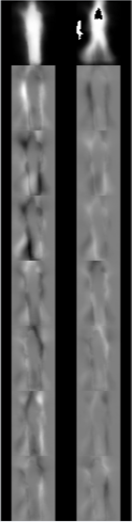
\includegraphics[width=.2\textwidth]{figs/Proposal_fig6a_RVQ_HMM_Weizmann_codebooks_8x2.png}}\hspace{0.3in}
								\subfigure[Test image.]{\includegraphics[width=.12\textwidth]{figs/Proposal_fig6b_RVQ_HMM_Weizmann_reconstruction2_goal.png}}\hspace{0.3in}
								\subfigure[RVQ testing, test image reconstruction using the decoder codebook.]{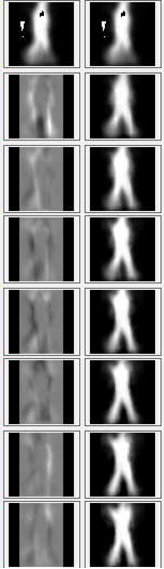
\includegraphics[width=0.228\textwidth]{figs/Proposal_fig6b_RVQ_HMM_Weizmann_reconstruction2.png}}
								\caption{Human action recognition, RVQ codebook and reconstruction.  With 2 code-vectors per stage, and 8 stages, a total of 256 reconstructed images are possible.  The left column in (c) shows the chosen stage code-vector, the right column shows progressive reconstruction.} 
							\label{fig:Weizmann_codebooks_and_reconstruction}		
								\end{figure}

%===================
\subsection{RVQ}
%===================
For action recognition, we have a set of labeled actions, i.e. a set of observations $O$ in the form of foreground segmented images as shown in Figure~\ref{fig:Weizmann_sequence}.  Our goal is to use RVQ to generate image descriptors that can be used to train one HMM model per action.  Our approach is summarized in the following lines and is illustrated graphically in Figure~\ref{fig:RVQ_HMM_IPCV2010_blockDiagram}:

\begin{enumerate}
\item \underline{Leave-one-out cross validation.}  We use leave-one-out cross-validation \cite{2000_JNL_SURVEYprml_Jain} by setting all action sequences of one user as test sequences.  This one time offline step takes approximately 6 minutes for 2400 images on a Core2 Duo 2.5 GHz laptop with 4GB RAM.

								\begin{figure}[t]	
								\centering
								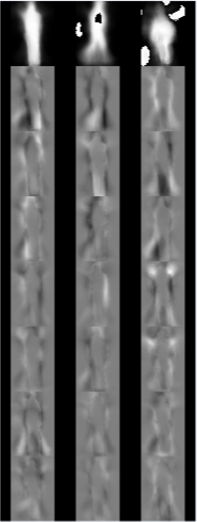
\includegraphics[width=0.28\textwidth]{figs/Proposal_fig6a_RVQ_HMM_Weizmann_codebooks_8x3.png}
								\caption{RVQ training, 8x3 decoder codebook.  The artefacts are due to image view clipping.  Notice that the first two stage code-vectors from the left for the top stage are quite similar for the 8x2 and 8x3 cases and seem to represent a standing and walking pose.}
							\label{fig:8x3_codebook}
								\end{figure}

\item \underline{RVQ training.}  An RVQ $\sigma$-tree is trained on the remaining users.  In this work, we use an 8x2 $\sigma$-tree, i.e. decoder codebook, since it gave good results without the complexity of having too many stage code-vectors per stage.  The trained 8x2 decoder codebook is shown in Figure~\ref{fig:Weizmann_codebooks_and_reconstruction}.  For reference, an 8x3 decoder codebook is shown in Figure~\ref{fig:8x3_codebook}.  

								\begin{figure}[t]	
								\includegraphics[width=1.0\textwidth]{figs/RVQ_HMM_IPCV2010_allActions.png}
								\caption{HMM testing (evaluation problem), log likelihoods of all actions of a single user.  Similar plots are generated for all users using leave-one-out cross-validation.  Results are then averaged and an action confusion matrix is generated.}
								\label{fig:RVQ_HMM_IPCV2010_allActions}
								\end{figure}

 
\item \underline{RVQ encoding (generating RVQ descriptor XDRs)}.  All training and test images are reconstructed using the decoder codebook.  An RVQ descriptor XDR $\mathbf{i}_{x_i}$ is generated for each of the training images $x_i$.  As explained in Section~\ref{subsec:RVQ}, each vector XDR is converted to a scalar value $\iota_{x_i}$.  Now, each training and test image is represented using a single scalar value.  For 2 code-vectors per stage, the descriptor ranges from 0 to 255, and a single byte is required to represent an entire image.  

%\item \underline{Train HMM}.  These training image descriptors can be used for classification in a manner similar to the training image projections in PCA analysis.  The RVQ based descriptors or PCA based projections can be used to create class conditional densities.  These densities can then be used for classification using maximum likelihood, or maximum aposteriori methods.  The processing time to create training image descriptors is about 3 minutes.  However, it is also an offline step.  The processing time includes GUI related instructions as well as SQL Server database access times.

								\begin{figure}[t]
								\centering	
								\subfigure[Our method \cite{2010_CNF_HMMRVQ_Aslam}]{\includegraphics[width=.50\textwidth]{figs/Proposal_fig7a_RVQ_HMM_Weizmann_TabularResults_us}\label{fig:Weizmann_TabularResults_us}}
								\subfigure[Gorelick et al. \cite{2007_JNL_SpaceTimeShapes_Gorelick}]{\includegraphics[width=0.45\textwidth]{figs/Proposal_fig7b_RVQ_HMM_Weizmann_TabularResults_gorelick}\label{fig:Weizmann_TabularResults_gorelick}}
								\subfigure[Manor et al. \cite{2001_CNF_EventBasedAnalysisVideo_Manor}]{\includegraphics[width=0.50\textwidth]{figs/Proposal_fig7c_RVQ_HMM_Weizmann_TabularResults_manor}\label{fig:Weizmann_TabularResults_irani}}
								\subfigure[Ali et al. \cite{2010_JNL_ActionReconKinematic_Ali}]{\includegraphics[width=0.45\textwidth]{figs/Proposal_fig7d_RVQ_HMM_Weizmann_TabularResults_shah}\label{fig:Weizmann_TabularResults_shah}}												
								\caption{Human action recognition, action confusion matrix.  The actions tested are: The 10 actions available are walk (a1), run (a2), skip (a3), jumping jacks (a4), jumping (a5), in-place jumping (a6), sideways motion (a7), waving with one hand (a8), waving with two hands (a9) and bending (a10).} 
								\label{fig:Weizmann_TabularResults}				
								\end{figure}
						
\item \underline{HMM inference (training)}.  Each action per user is composed of a sequence of images, which are now represented as a sequence of scalar XDR values.  For a single action, scalar descriptor sequences for each training user are used to train an HMM model $\lambda$.  The number of HMM models trained is equal to the number of actions.  This step takes around 700 msec in Matlab.  All previous steps were executed in the C language.

\item \underline{HMM evaluation (testing)}.  Using leave-one-out cross-validation, the actions of a single user are tested against all HMM models.  A log likelihood is generated per action per user.  The label of the action corresponding to the HMM model that generates the largest log likelihood is tagged to each action sequence.  The results of all actions tested for a single test user are shown in Figure~\ref{fig:RVQ_HMM_IPCV2010_allActions}.  Similar results are generated for all users.  This step is then repeated for all users in the database using the leave one out procedure.  This step takes 1.1 msec per frame in Matlab.   
\end{enumerate}

%===========================
\subsection{Results}
%===========================
The steps in the previous section are repeated for all actions of each user.  Correct recognition scores for each action are averaged and displayed in Figure~\ref{fig:Weizmann_TabularResults}.  Also displayed in this figure are recognition rates obtained by other researchers for this same dataset.

For the number of HMM states $N$, different values were tried.  Empirical testing revealed that $N=4, 5, 6$ produce good results.  A value of $N=4$ was chosen.  It is expected that the reason for this is that there are around 4 dominant poses over all actions, (a) upright posture which is used in most actions, (b) a slightly bent posture for actions such as bending, jumping, skipping, (c) arms forward posture for walking, running, and (d) arms up posture for waving and jumping jacks.

The results obtained with our low computational complexity method compare favorably with other methods reported in the literature.  There is a correlation in recognition accuracy with \cite{2007_JNL_SpaceTimeShapes_Gorelick} for all actions except these four:  

\begin{itemize}
\item Bending (a1) which is confused with sideways motion (a7)
\item Skipping (a3) which is confused with running (a2)
\item Jumping jacks (a4), the most ambiguous action, which are confused with two-hand waving (a9)
\item In place-jumping (a6) which is confused with one-hand waving (a8)
\end{itemize}

For both our method and the method in \cite{2007_JNL_SpaceTimeShapes_Gorelick}, jumping (a5) is confused with skipping (a3).  Our method produces better results for running (a2), one-hand waving (a8), two-hand waving (a9) and bending (a10).  

Overall, it is encouraging that a straightforward application of HMM on RVQ processed image sequences produces such high recognition rates.  It is expected that better recognition rates can be achieved with using more stages or number of code-vectors per stage.  Moreover, more research into better RVQ codebook design methods is expected to further improve recognition rates.  

In this chapter, we focused on understanding the usage of RVQ in computer vision in face and action recognition applications.  We transitioned from using images to image sequences.  The usage of image sequences is particularly important since this is the first reported application of RVQ on image sequences.  However, in both cases discussed in this chapter, the RVQ codebook is static.  In the next chapter, we further our application and understanding of RVQ by allowing the codebook itself to evolve dynamically.

\end{Body}
%##############################################################################################################
\begin{EndMatter}
\references 				%generates the bibliography page
\end{EndMatter}
\end{document}
%##############################################################################################################
